\documentclass[tikz,border=2pt]{standalone}
\usepackage{pgfplots}
\pgfplotsset{compat=1.18}
\begin{document}
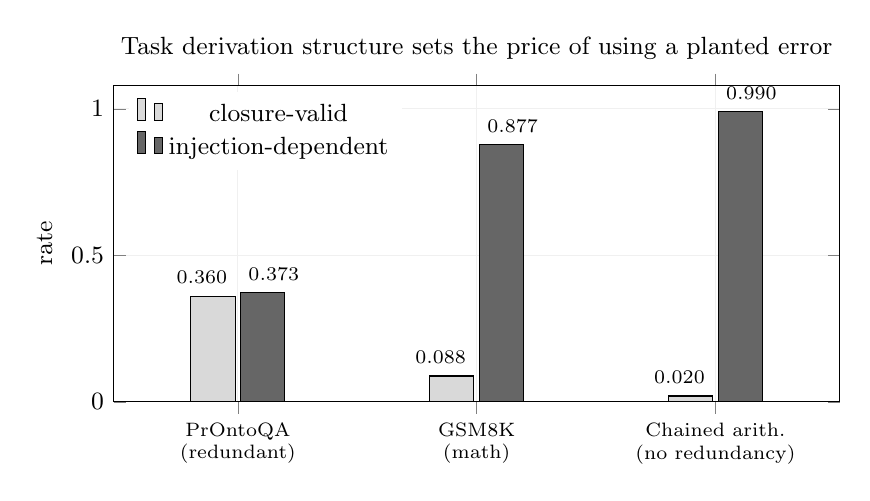
\begin{tikzpicture}
\begin{axis}[
  ybar,width=10.8cm,height=5.6cm,bar width=16pt,
  ymin=0,ymax=1.08,ylabel={rate},
  symbolic x coords={PrOntoQA,GSM8K,Chained},
  xtick=data,
  xticklabels={PrOntoQA\\(redundant),GSM8K\\(math),Chained arith.\\(no redundancy)},
  xticklabel style={align=center,font=\scriptsize,text width=2.7cm},
  tick label style={font=\small},label style={font=\small},
  title={Task derivation structure sets the price of using a planted error},
  title style={font=\small},
  legend style={at={(0.02,0.98)},anchor=north west,draw=none,font=\small},
  nodes near coords={\pgfmathprintnumber[fixed,zerofill,precision=3]{\pgfplotspointmeta}},
  nodes near coords style={font=\scriptsize,text=black},
  point meta=y,
  enlarge x limits=.26,grid=both,grid style={gray!12},
]
\addplot+[black,fill=black!15,draw=black,
  nodes near coords style={font=\scriptsize,text=black,anchor=south,xshift=-4pt,yshift=1pt}
] coordinates {
  (PrOntoQA,0.360) (GSM8K,0.088) (Chained,0.020)
};
\addlegendentry{closure-valid}
\addplot+[black,fill=black!60,draw=black,
  nodes near coords style={font=\scriptsize,text=black,anchor=south,xshift=4pt,yshift=1pt}
] coordinates {
  (PrOntoQA,0.373) (GSM8K,0.877) (Chained,0.990)
};
\addlegendentry{injection-dependent}
\end{axis}
\end{tikzpicture}
\end{document}
